% \documentclass[12pt]{article}
\documentclass[useAMS,referee,usenatbib]{biom}
%\usepackage[utf8]{inputenc}
%\usepackage{amsmath, authblk}
\usepackage{amsmath}
%\usepackage{amsthm}
\usepackage{amsfonts}
\usepackage{amssymb}
\usepackage{multirow}
\usepackage{comment}
\usepackage{lscape} 
%\usepackage{graphics}
%\usepackage{afterpage}
%\usepackage{xcolor}
%\usepackage{citeppp}
%\usepackage[usenatbib]{natbib}
%\usepackage[round]{natbib}
%\usepackage{url} 
\usepackage{graphicx}
%\usepackage{subcaption}

%\usepackage[margin = 1in]{geometry}

\usepackage[figuresright]{rotating}

\DeclareMathOperator*{\argmax}{arg\,max}
\DeclareMathOperator*{\argmin}{arg\,min}
%\def\bs{\boldsymbol}
\def\bs{\bmath}
\def\bb{\mathbb}


\newtheorem{prop}{Proposition}
%\newtheorem{lemma}{Lemma}



\title[Empirical Bayes Covariance Matrix Estimation]{A Compound Decision Approach to Covariance Matrix Estimation}

\author{Huiqin Xin$^{*}$\email{huiqinx2@illinois.edu } and
Sihai Dave Zhao$^{**}$\email{sdzhao@illinois.edu} \\
Department of Statistics, University of Illinois at Urbana-Champaign, Champaign, Illinois}
%
%\author{John Author$^{*}$\email{author@address.edu} and
%Kathy Authoress$^{**}$\email{email2@address.edu} \\
%Department of Statistics, University of Warwick, Coventry CV4 7AL, U.K.}

\begin{document}

%\date{{\it Received October} 2007. {\it Revised February} 2008.  {\it
%Accepted March} 2008.}

\label{firstpage}
\begin{abstract}
  We propose an empirical Bayes method to estimate high-dimensional covariance matrices. Our procedure centers on vectorizing the covariance matrix and treating matrix estimation as a vector estimation problem. Drawing from the compound decision theory literature, we introduce a new class of decision rules that generalizes several existing procedures. We then use a nonparametric empirical Bayes $g$-modeling approach to estimate the oracle optimal rule in that class. This allows us to let the data itself determine how best to shrink the estimator, rather than shrinking in a pre-determined direction such as toward a diagonal matrix. Simulation results and a gene expression network analysis shows that our approach can outperform a number of state-of-the-art proposals in a wide range of settings, sometimes substantially.
\end{abstract}

\begin{keywords}
Compound decision theory; $g$-modeling; nonparametric maximum likelihood; separable decision rule.
\end{keywords}

\maketitle

\section{Introduction}
\label{introduction}

Covariance matrix estimation is a fundamental statistical problem that plays an essential role in various applications, such as portfolio management \citep{ledoit2003improved}, genomics \citep{schafer2005shrinkage}, and array signal processing \citep{abramovich2001locally}. However, in modern problems the number of features can be of the same order as or exceed the sample size, and the standard sample covariance matrix estimator behaves poorly in this regime. To overcome these issues, various methods have been developed to estimate high-dimensional covariance matrix. These can roughly be divided into two groups, according to whether they impose assumptions about the structure of population covariance matrix.

Structured methods make structural assumptions about the population covariance matrix. One class models the population covariance matrix as sparse. The most common method to address this problem is thresholding \citep{rothman2009generalized, cai2011adaptive}. Penalized likelihood methods \citep{xue2012positive} can also estimate large-scale sparse covariance matrix by penalizing a log-likelihood function. Another class of methods assume the data arise from a factor model \citep{fan2008high}, so that the covariance matrix has low intrinsic dimension. Other common structured methods assume that the covariance matrix is banding \citep{li2017estimation} or Toeplitz matrix \citep{liu2017covariance}. 

In contrast, unstructured methods do not make any assumptions about the population covariance matrix, yet can still outperform the sample covariance matrix. A first example was the linear shrinkage approach of \citet{ledoit2004well}, which shrinks the sample covariance matrix toward a scaled identity matrix. More recently, nonlinear shrinkage methods were developed \citep{ledoit2012nonlinear, ledoit2019quadratic, lam2016nonparametric}. These shrink the eigenvalues of the sample covariance matrix toward clusters. Linear shrinkage can be viewed as a special case of nonlinear shrinkage, as it shrinks sample eigenvalues toward their global mean.

Nonlinear shrinkage estimators have desirable optimality properties \citep{ledoit2018analytical} and show excellent performance. However, they modify only the sample eigenvalues and not the sample eigenvectors. It is known that sample eigenvectors are not consistent estimators of population eigenvectors when the dimension and the sample size increase at the same rate \citep{mestre2008asymptotic}. This suggests that there may exist a class of unstructured estimators that can outperform nonlinear shrinkage.

%In this paper, we propose a new covariance matrix estimator which is approximately optimal among all separable estimators. Our method is motivated by the similarity between covariance estimation and vector mean estimation. Covariance matrix estimation under Frobenius loss can be viewed as a vector estimation problem by converting the matrix to a vector. \citep{cai_liu} used this motivation to generalize thresholding method in mean vector estimation to large sparse covariance matrix estimation. Nevertheless, they are not totally the same because covariance matrix has repeated entries due to its symmetry. In mean vector estimation problem, optimality has been achieved among all separable decision rules. \citep{jiang_zhang2009} and \citep{brown_greenshtein} proposed empirical Bayes methods to approximate the optimal separable estimator. We proposed to apply vector estimation methods to covariance estimation problem and expect that these methods will also have good properties here. Result in simulation and real data set shows that our estimator has good performance in different scenarios.

Here we propose a new unstructured estimator for high-dimensional covariance matrices. Our approach centers on vectorizing the covariance matrix and treating matrix estimation as a vector estimation problem. We do this because it allows us to use a nonparametric empirical Bayes shrinkage procedure, which has been shown in the compound decision literature to have excellent properties \citep{jiang2009general, koenker2014convex}. We then reassemble the estimated vector into matrix form and project onto the space of positive-definite matrices to give our final estimator. Surprisingly, though our vectorized approach essentially ignores the matrix structure, it can still substantially outperform a number of state-of-the-art proposals in simulations and a real data analysis.

The article is organized as follows. In Section \ref{sec:method}, we briefly review compound decision theory and then introduce our proposed approach. In Section \ref{numerical results} we illustrate the performance of our method in simulations and a gene expression dataset. Finally, Section \ref{sec:discussion} concludes with a discussion. Our procedure is implemented in the R package \verb|cole|, available on GitHub.

\section{\label{sec:method}Method}
\subsection{\label{sec:compound}Compound decision problem formulation}
Suppose we have $n$ observations $\bs{X}_1,\ldots,\bs{X}_n$ independently generated from a $p$-dimensional $\mathcal{N}(\bs{0},\bs{\Sigma})$. The purpose of this paper is to find an estimator $\bs{\delta}(\bs{X})$ of $\bs{\Sigma}$ that minimizes the scaled squared Frobenius risk
\begin{equation}
\label{frobenius risk}
R(\bs{\Sigma}, \bs{\delta}) = \frac{1}{p^2} \sum_{j,k=1}^p \mathbb{E}[\{\delta_{jk}(\bs{X})-\sigma_{jk}\}^2],
\end{equation}
where $\sigma_{jk}$ is the $jk$th entry of $\bs{\Sigma}$ and $\delta_{jk}(\bs{X})$ is its corresponding estimate.

Our proposed approach is motivated by two observations. First, \ref{frobenius risk} shows that estimating $\bs{\Sigma}$ under Frobenius risk is equivalent to simultaneously estimating every component of the vector $(\sigma_{11},\ldots,\sigma_{pp})^\top$ under a loss function that aggregates errors across components. Second, this type of vector estimation problem has been well-studied in the compound decision literature. Thus, recent advances in vector estimation may be profitably applied to covariance matrices.

We first briefly review compound decision problems. Introduced by \citet{robbins1951asymptotically}, these problems study the simultaneous estimation of multiple parameters $\bs{\theta} = (\theta_1, \ldots, \theta_n)^\top$ given data $\bs{Y} = (Y_1, \ldots, Y_n)^\top$, with $Y_i\sim P_{\theta_i}$. Specifically, the goal is to develop a decision rule $\bs{\delta}(\bs{Y}) = (\delta_1(\bs{Y}),\ldots,\delta_n(\bs{Y}))$ that minimizes the compound risk
\begin{equation}
\label{compound risk}
R(\bs{\theta},\bs{\delta}) = \frac{1}{n}\sum_{i=1}^n \bb{E} L(\theta_i,\delta_i(\bs{Y}))
\end{equation}
where $L$ is a loss function measuring the accuracy of $\delta_i(\bs{Y})$ as an estimate of $\theta_i$. A classical example is the homoscedastic Gaussian sequence problem, where $Y_i \sim N(\theta_i, 1)$ independently and $L(t, d) = (t - d)^2$ is squared error loss \citep{johnstone2017gaussian}.

A key property of compound decision problems is that while a given $Y_i$ seems to offer no information about any specific $\theta_j$ when $j \ne i$, borrowing information across all components of $\bs{Y}$ to estimate $\bs{\theta}$ is superior to estimating each $\theta_i$ using the corresponding $Y_i$ alone. A classical example of this phenomenon is the James-Stein estimator \citep{james1961estimation}, which estimates $\bs{\theta}$ in the Gaussian sequence problem by shrinking each $Y_i$ toward $0$ by a factor that depends on all components of $\bs{Y}$. It is well-known that when $n \geq 3$, the James-Stein estimator dominates the maximum likelihood estimator, which simply estimates $\bs{\theta}$ using $\bs{Y}$. A long line of subsequent work has led to much more sophisticated and accurate procedures for estimating $\bs{\theta}$ \citep{brown2009nonparametric, jiang2009general, johnstone2017gaussian, lindley1962discussion, fourdrinier2018shrinkage}.

We propose to apply some of these recent vector estimation ideas to covariance matrix estimation. Clearly, covariance matrix estimation under the Frobenius risk \ref{frobenius risk} can be viewed as a compound decision problem. Furthermore, some existing covariance matrix estimation procedures can already be interpreted as taking a vector approach. The sample covariance matrix $\bs{S}$, for instance, can be thought of as estimating each component of $(\sigma_{11},\ldots,\sigma_{pp})^\top$ using maximum likelihood. Less trivially, \citet{cai2011adaptive} studied sparse high-dimensional covariance matrices and explicitly appealed to the vector perspective. Their adaptive thresholding method is a version of the soft thresholding method of \citet{donoho1995adapting}, which was originally developed to estimate a sparse mean vector in the Gaussian sequence problem.

Interestingly, we can also show that the celebrated linear shrinkage covariance matrix estimator of \citet{ledoit2004well} can be interpreted as a vector estimator. The estimator is defined as
\begin{equation}
\label{linear model}
\widehat{\bs{\Sigma}}_{\text{LW}} = \widehat{\rho}_{\text{LW}} \bs{S} + (1-\widehat{\rho}_{\text{LW}})\widehat{\mu} \bs{I}
\end{equation} 
where $\widehat{\mu} = \text{tr}(\bs{S})/p$, and $\widehat{\rho}_{\text{LW}} = 1 - b_n^2 / d_n^2$ for $d_n^2=\|\bs{S}-\widehat{\mu} \bs{I} \|_F^2$ and $b_n^2 = \sum_{i=1}^n \| \bs{X}_i \bs{X}_i^\top - \bs{S} \|_F^2 / n^2$. Now consider the problem of estimating the vectorized $\bs{\Sigma}$ under risk \ref{frobenius risk}. We restrict attention to decision rules that estimate each component $\sigma_{jk}$ using
\begin{equation}
  \label{linear class}
  \beta_S s_{jk} + \beta_I u_{jk},
\end{equation}
where $s_{jk}$ is the $jk$th entry of $\bs{S}$, $u_{jk}$ is the $jk$th entry of $\bs{I}$, and the class is indexed by the parameters $(\beta_S, \beta_I)$. It is straightforward to show that
$$\widehat{R}(\beta_S,\beta_I) = \frac{1}{p^2} \sum_{j,k=1}^{p}[(2\beta_S-1) \widehat{\Delta}_{jk}^2 + \{(1- \beta_S) s_{jk} - \beta_I u_{jk}\}^2 ]$$
is an unbiased estimate of the risk \ref{frobenius risk}, where $\widehat{\Delta}_{jk}^2 = \sum_{i=1}^{n}(X_{ij}X_{ik}-s_{jk})^2 / n$ is the sample variance of $s_{jk}$. The optimal estimator in this class can now be chosen by minimizing $\widehat{R}(\beta_S, \beta_I)$ over $\beta_S$ and $\beta_I$. It can be shown that this is equivalent to estimating the vector $(\sigma_{11}, \ldots, \sigma_{pp})^\top$ by shrinking $(s_{11}, \ldots, s_{pp})^\top$ toward the one-dimensional subspace spanned by $(u_{11}, \ldots, u_{pp})^\top$ \citep{biscarri2019thesis, lindley1962discussion}. Proposition \ref{prop:linear} shows that this subspace shrinkage estimator is identical to the \citet{ledoit2004well} estimator \ref{linear model}.
\begin{prop}
  \label{prop:linear}
  Define the estimator $\widehat{\bs{\Sigma}}_V$ such that its $jk$th entry obeys $\widehat{\sigma}_{jk} = \widehat{\beta}_S s_{jk} + \widehat{\beta}_I u_{jk}$, where $(\widehat{\beta}_S, \widehat{\beta}_I) = \argmin_{\beta_S, \beta_I} \widehat{R}(\beta_S, \beta_I)$. Then $\widehat{\bs{\Sigma}}_V$ = $\widehat{\bs{\Sigma}}_{LW}$.
\end{prop}

\subsection{\label{sec:proposed}Proposed estimator}

The previous section argues that treating covariance matrix estimation as a vector estimation problem can be a fruitful strategy, but discusses only estimators linear in $s_{jk}$. We propose to consider a larger class, the class of so-called separable rules. In the standard compound decision problem of estimating $\bs{\theta}$ using $\bs{Y}$, a separable decision rule $\bs{\delta}(\bs{Y})$ is one where $\delta_i(\bs{Y}) = t(Y_i)$ \citep{robbins1951asymptotically}. Here we generalize this to the problem of estimating a vectorized matrix. For decision rules $\bs{\delta}(\bs{X}) = (\delta_{11}(\bs{X}),\ldots,\delta_{pp}(\bs{X}))$ that estimate $(\sigma_{11}, \ldots, \sigma_{pp})^\top$, define the class of separable rules
\begin{equation}
  \label{separable}
  \mathcal{S} = \{\bs{\delta} : \delta_{jk} = t(\bs{X}_{\cdot j}, \bs{X}_{\cdot k}), j\neq k,\quad 
   \delta_{jj} = \widetilde{t}(\bs{X}_{\cdot j}),j=1,\ldots,p)\},
\end{equation}
where $\bs{X}_{\cdot j} = (X_{1j}, \ldots, X_{nj})^\top$ is the vector of observed values of the $j$th feature. In other words, rules in $\mathcal{S}$ estimate the $jk$th entry of the covariance matrix using a fixed function $t$ of only observations from features $j$ and $k$. The sufficient statistics of $(\bs{X}_{\cdot j}, \bs{X}_{\cdot k})$ is $2\times 2$ matrix
$\begin{bmatrix}
s_{jj} & s_{jk} \\
s_{kj} & s_{kk} 
\end{bmatrix}$.


We propose to search for the optimal estimator within $\mathcal{S}$. This is sensible because $\mathcal{S}$ includes the sample covariance $(s_{11}, \ldots, s_{pp})^\top$, the class of linear estimators \ref{linear class} used by \citet{ledoit2004well}, which can be expressed as
\[
\delta_{jk}(\bs{X}) = \beta_S \bs{X}_{\cdot j}^\top \bs{X}_{\cdot k} / n + \beta_I I(\bs{X}_{\cdot j} = \bs{X}_{\cdot k}),
\]
and the class of adaptive thresholding estimators for sparse covariance matrices studied by \citet{cai2011adaptive}. Therefore the optimal separable estimator $\bs{\delta}^\star$ that minimizes the scaled squared Frobenius risk \ref{frobenius risk} will perform at least as well as these three estimators, and may perform better. Targeting the optimal separable rule is standard in the compound decision literature \citep{zhang2003compound}.

The optimal $\bs{\delta}^\star$ is an oracle estimator and cannot be calculated in practice, as the true risk is unknown. In the classical compound decision framework, empirical Bayes methods are used to estimate the oracle optimal separable rule \citep{robbins1955empirical, zhang2003compound, brown2009nonparametric, jiang2009general, efron2014two, efron2019bayes}. We take a similar approach here. To simplify notation, denote $(\bs{X}_{\cdot j}, \bs{X}_{\cdot k})^\top$ as $\bs{A}_{jk}$. $f(\cdot \mid \bs{\eta}_{jk})$, the density of $\bs{A}_{jk}$, depends on $\bs{\eta}_{jk} = (\sigma_j, \sigma_k, r_{jk})^\top$, where $\sigma_j$ and $\sigma_k$ are the true standard deviations of the $j$th and $k$th covariates and $r_{jk} = \sigma_{jk} / (\sigma_j \sigma_k)$ is their true correlation. When $r_{jk} \ne 1$, $\bs{A}_{jk}$ is comprised of $n$ independent mean-zero multivariate normals with covariance matrices
\[
\bs{C}_{jk}=\begin{bmatrix}
&\sigma_j^2 & \sigma_j\sigma_k r_{jk} \\
& \sigma_j\sigma_k r_{jk}  & \sigma_k^2
\end{bmatrix}.
\]
When $r_{jk} = 1$, $\bs{A}_{jk}$ consists of mean-zero univariate normals with variances $\sigma_j^2$.

Now consider the Bayesian model for non-diagonal entries
\begin{equation}
  \label{bayesian nondiagonal}
  \bs{A} \mid \bs{\eta} \sim f(\cdot \mid \bs{\eta}),
  \quad
  \bs{\eta} \sim G_{nd}(a,b, \gamma) =  \frac{2}{p(p-1)} \sum_{1\leq k<j\leq p} I(\sigma_j \leq a, \sigma_k \leq b, r_{jk} \leq \gamma).
\end{equation}
and diagonal entries
\begin{equation}
  \label{bayesian diagonal}
  \bs{A} \mid a \sim \widetilde{f}(\cdot \mid a),
  \quad
  a \sim G_d(a) =  \frac{1}{p} \sum_{j=1}^p I(\sigma_j \leq a).
\end{equation}
By the fundamental theorem of compound decisions \citep{robbins1951asymptotically, jiang2009general}, this is closely related to the vectorized covariance matrix estimation problem under Frobenius risk \ref{frobenius risk}: for any separable $\bs{\delta} \in \mathcal{S}$ \ref{separable}, the Frobenius risk can be written as
\begin{align*}
  R(\bs{\Sigma}, \bs{\delta})
  =\,&
  \frac{1}{p^2} \{\sum_{1\leq k<j\leq p}^p
  \int \{t(\bs{A}) - \sigma_{jk} \}^2 f(\bs{A} \mid \bs{\eta}_{jk}) d\bs{A} 
  +
  \sum_{j=1}^p
  \int \{\widetilde{t}(\bs{X}) - \sigma_{jj} \}^2 \widetilde{f}(\bs{X} \mid s_{jj}) d\bs{X}
  \}\\
  =\,&
  \frac{p-1}{p}\int \int \{t(\bs{A}) - g(\bs{\eta})\}^2 f(\bs{A} \mid \bs{\eta}) dG_{nd}(\bs{\eta}) d\bs{A}
  +
  \frac{1}{p}\int \int \{\widetilde{t}(\bs{X}) - a^2\}^2 \widetilde{f}(\bs{X} \mid a) dG_{d}(a) d\bs{X} \\
  =\,&
   \frac{p-1}{p}\bb{E}[\{t(\bs{A}) -  g(\bs{\eta})\}^2]+ \frac{1}{p}\bb{E}[\{\widetilde{t}(\bs{X}) -  a^2\}^2],
\end{align*}
where $g(a, b, \gamma) = a b \gamma$ and the final expectation is the Bayes risk of estimating $\sigma_{jk}$. The optimal oracle separable rule $\bs{\delta}^\star$ therefore has $jk$th entry equal to $\delta^\star_{jk}(\bs{X}) = t^\star(\bs{A}_{jk})$ for $j\neq k$ and $\delta^\star_{jj}(\bs{X}) = \widetilde{t}^\star(\bs{X}_{\cdot j})$, where $t^\star = \mathbb{E}\{g(\bs{\eta}) \mid \bs{A}\}$ and $\widetilde{t}^\star = \mathbb{E}\{g(a) \mid \bs{X}\}$ minimizes the Bayes risk.

Based on this result, we propose the following empirical Bayes procedure. We first use nonparametric maximum likelihood \citep{kiefer1956consistency} to estimate the prior $G_p$. Under the Bayesian model \ref{bayesian}, and the working assumption that the $\bs{A}_{jk}$ are independent across $jk$, we estimate $G_{nd}$ using
\begin{equation}
  \label{Gnd hat}
  \widehat{G}_{nd} = \argmax_{G \in \mathcal{G}_{nd}} \prod_{1\leq k<j<p} \int f(\bs{A}_{jk} \mid \bs{\eta}) dG(\bs{\eta}),
\end{equation}

estimate $G_d$ using
\begin{equation}
  \label{Gd hat}
  \widehat{G}_d = \argmax_{G \in \mathcal{G}_d} \prod_{j = 1}^p \int \widetilde{f}(\bs{X} \mid a) dG(a),
\end{equation}
where $\mathcal{G}_{nd}$ is the family of all distributions supported on $\mathbb{R}_+ \times \mathbb{R}_+ \times [-1, 1]$,   $\mathcal{G}_{d}$ is the family of all distributions supported on $\mathbb{R}$. Of course, the $\bs{A}_{jk}$ are not independent, so $\widehat{G}_p$ does not maximize a likelihood but rather a pairwise composite likelihood \citep{varin2011overview}. Using $\widehat{G}_p$, we estimate the vectorized $\bs{\Sigma}$ using $ \widehat{\bs{\delta}}(\bs{X})
  =
  (\widehat{t}(\bs{A}_{21}), \ldots,  \widehat{t}(\bs{A}_{p,p-1}),\widehat{t}(\bs{X}_{\cdot 1}),\ldots,\widehat{t}(\bs{X}_{\cdot p}))$, where 
\begin{equation}
  \label{proposed}
  \widehat{t}(\bs{A}_{jk}) = \frac{\int g(\bs{\eta}) f(\bs{A}_{jk} \mid \bs{\eta})d\widehat{G}_{nd}(\bs{\eta})}{\int f(\bs{A}_{jk} \mid \bs{\eta}) d\widehat{G}_{nd}(\bs{\eta})},
  \quad 
  \widehat{t}(\bs{X}_{\cdot j}) = \frac{\int a^2 \widetilde{f}(\bs{X}_{\cdot j} \mid a)d\widehat{G}_d(a)}{\int \widetilde{f}(\bs{X}_{\cdot j} \mid a) d\widehat{G}_d(a)}.
\end{equation}
The $\widehat{t}$ estimates the Bayes rule $t^\star$ and $\widehat{\bs{\delta}}$ estimate the optimal oracle separable rule $\bs{\delta}^\star$.

Our proposed procedure is an example of what \citet{efron2014two} calls $g$-modeling, an approach to empirical Bayes problems that proceeds by modeling the prior. A major advantage of nonparametric estiation of the prior is that it allows the data itself to determine how best to shrink the estimator. In contrast, most existing methods shrink in a pre-determined direction, such as toward a diagonal matrix in the case of \citet{ledoit2004well}. Theoretical justification of our proposed $\widehat{\bs{\delta}}$ is difficult and is discussed in Section \ref{discussion}. Nevertheless, our numerical results in Section \ref{numerical results} show that in practice, our $\widehat{\bs{\delta}}$ can outperform many existing covariance matrix estimators.

\subsection{\label{implementation}Implementation}

Calculating the estimated prior $\widehat{G}_p$ \ref{Gp hat} is difficult, as it is an infinite-dimensional optimization problem over the class of all probability distributions $\mathcal{G}$. \citet{lindsay1983geometry} showed that the solution is atomic and is supported on at most $p^2$ points. The EM algorithm has traditionally been used to estimate the locations of the support points and the masses at those points \citep{laird1978nonparametric}, but this is a difficult nonconvex optimization problem.

Instead, we maximize the pairwise composite likelihood over a fixed grid of support points, similar to recent $g$-modeling procedures for standard compound decision problems; this restores convexity \citep{jiang2009general, koenker2014convex, feng2018approximate}. Specifically, we assume that the prior for the $\bs{\eta}_{jk} = (\sigma_j, \sigma_k, r_{jk})^\top$ is supported on $D$ fixed support points $\bs{\xi}_{\tau}$, $\tau=1,\ldots, D$. We can then use the EM algorithm to estimate the masses $\widehat{\bs{w}}=\{\widehat{w}_{1},\ldots, \widehat{w}_{D}\}$ at those points via the iteration
\[
\widehat{w}_{\tau}^{(k)} = \frac{1}{p^2}\sum_{j, k = 1}^p \frac{\widehat{w}_{\tau}^{(k-1)} f(\bs{A}_{jk} \mid \bs{\xi}_{\tau})}{\sum_{l=1}^D\widehat{w}_l^{(k-1)} f(\bs{A}_{jk} \mid \bs{\xi}_l)}
\]
over $k$. Early stopping of the EM algorithm can be useful \citep{koenker2019comment}, and more sophisticated convex optimization procedures can be used as well \citep{koenker2014convex}. Our proposed estimator \ref{proposed} then becomes
\[
\widehat{t}(\bs{A}_{jk}) = \frac{ \sum_{\tau=1}^D g(\bs{\xi}_\tau) f(\bs{A} \mid \bs{\xi}_\tau) \widehat{w}_{\tau}}{ \sum_{\tau=1}^D f(\bs{A} \mid \bs{\xi}_\tau) \widehat{w}_{\tau}},
\quad
\widehat{t}(\bs{X}_{\cdot j}) = \frac{ \sum_{\tau=1}^D a_{\tau}^2 \widetilde{f}(\bs{X}_{\cdot j} \mid a_\tau) \widehat{w}_{\tau}}{ \sum_{\tau=1}^D \widetilde{f}(\bs{X}_{\cdot j}  \mid a_\tau) \widehat{w}_{\tau}}.
\]

Ideally, the grid points should be chosen to densely cover the parameter space. However, the fact that $G_p$ is multivariate poses difficulties, as for example using a grid of $d$ points in each dimension requires a total of $D = d^3$ grid points, which requires huge computational cost for even moderate $d$. Alternatively, we can use a so-called exemplar algorithm \citep{saha2020nonparametric}, which sets the support points to equal the observed sample versions $\widehat{\bs{\eta}}_{jk}$ of the $\bs{\eta}_{jk}$. This reduces the size of the support set, but even in this case the computation complexity grows like $O(p^2)$.

Here we propose a clustering-based exemplar algorithm to further improve computational efficiency. Let $s_j$, $s_k$, and $\gamma_{jk}$ be the sample variances and correlation between the $j$th and $k$th covariates. We first apply $K$-means clustering to identify $K$ clusters among the $p (p-1) / 2$ off-diagonal sample points $(s_j,s_k,\gamma_{jk})$ and $\lceil{K^{1/2}}\rceil$ clusters among the $p$ diagonal sample points $(s_j,s_j,1)$. We then use the $K+\lceil{K^{1/2}}\rceil$ cluster centroids as our support points. We cluster the off- and on-diagonal observations separately to ensure that the support points $\bs{\xi}_\tau$ are such that $f(\bs{A}_{jk} \mid \bs{\xi}_\tau) \ne 0$ when both $j = k$ and $j \ne k$. Figure \ref{fig:sim1_frobenius} shows that different $K$ have similar estimation accuracy compared to the exemplar algorithm, while Table \ref{tab:sim1_time} shows that they can be significantly faster.

In our implementation, we use the density function of $\bs{S}_{jk}=\begin{bmatrix}
s_{jj} & s_{jk} \\
s_{kj} & s_{kk} 
\end{bmatrix}$ instead of $\bs{A}_{jk}$ since it is the sufficient statistics of $\bs{A}_{jk}$ and easier to calculate. Based on the property of sufficient statistics, 
\begin{equation}
\frac{f(\bs{A}_{jk}\mid \bs{\xi}_{\tau})}{f(\bs{A}_{jk}\mid \bs{\xi}_l)} = \frac{f(\bs{S}_{jk}\mid \bs{\xi}_{\tau})}{f(\bs{S}_{jk}\mid \bs{\xi}_l)}
\end{equation}
So it is equivalent to use $f(\bs{A}_{jk}\mid \bs{\xi}_{\tau})$ in calculation.
\subsection{\label{posdef}Positive definiteness correction}
Our proposed estimator \ref{proposed} is not guaranteed to be positive-definite. To correct this, we reshape our vector estimator back into a matrix and then identify the closest positive-definite matrix. \citet{higham1988computing} and \citet{huang2017calibration} showed that the projection of a $p \times p$ symmetric matrix $\bs{B}$ onto the space of positive semi-definite matrices is
\[
P_0(\bs{B})
=
\argmin_{\bs{A}\geq 0} \Vert\bs{A}-\bs{B}\Vert
=
\bs{Q}\text{diag}\{\max(\lambda_1,0),\max(\lambda_2,0),\ldots,\max(\lambda_p,0)\}\bs{Q}^\top,
\]
where $\Vert \cdot \Vert$ denotes the Frobenius norm, $\bs{Q}$ is the matrix of eigenvectors of $\bs{B}$, and $\lambda_1,\ldots,\lambda_p$ are its eigenvalues. 

To guarantee positive-definiteness, we follow \citet{huang2017calibration} and replace non-positive eigenvalues with a chosen positive value $c$ smaller than the least positive eigenvalue $\lambda_{\min}^+$, so that the corrected estimate is
\begin{equation}
  \label{near posdef}
  P_0(\bs{B})
  =
  \bs{Q}\text{diag}\{\max(\lambda_1,c),\max(\lambda_2,c),\ldots,\max(\lambda_p,c)\}\bs{Q}^\top.
\end{equation}
\citet{huang2017calibration} suggest $c_{\alpha}=10^{-\alpha}\lambda_{\min}^+$, where the parameter $\alpha$ is chosen to minimize $\Vert B - P_{c_{\alpha}}(B) \Vert + \alpha$ over a uniform partition of $\{\alpha_1,\ldots,\alpha_K\}$ of $[0,\alpha_K]$. In this paper we chose $K=20$ and $\alpha_K=10$.


\section{\label{numerical results}Numerical Results}
\subsection{\label{models}Models}

We considered five models for the population covariance matrix. For the first four settings, $\bs{\Sigma} = \text{diag}(\bs{s}) \bs{C} \text{diag}(\bs{s})$, where $\bs{C}$ is correlation matrix and $\bs{s}$ is a vector of standard deviations.
\begin{itemize}
\item Model 1. The standard deviations were independently generated from $\mathcal{U}(1,1.5)$ and the correlation matrix followed Model 2 of \citet{cai2011adaptive}:
  \[
  \bs{C}=
  \begin{pmatrix}&\bs{A}_1 & \bs{0} \\ &\bs{0} &\bs{I}_{p/2\times p/2}\end{pmatrix},
  \]
  where the $jk$th entry of $\bs{A}_1$ is $a_{jk} = \max(1- \vert j - k \vert / 10, 0)$. This setting modeled a sparse covariance matrix.
  
\item Model 2. The first $p / 2$ standard deviations equaled 1, the last $p / 2$ equaled 2, and the correlation matrix was
  \[
  \bs{C} = \begin{pmatrix} & \bs{C}_{11} & \bs{C}_{12} \\  & \bs{C}_{21} & \bs{C}_{22}\end{pmatrix},
  \]
  where $\bs{C}_{11}$ and $\bs{C}_{22}$ were $p/2 \times p/2$ compound symmetric matrices with correlation parameters 0.8 and 0.2, respectively, and $\bs{C}_{12}$ and $\bs{C}_{21}$ were $p/2 \times p/2$ matrices with entries equal to 0.4. This model was designed such that larger $\sigma_j$ and $\sigma_k$ tended to correspond to larger $r_{jk}$.
  
\item Model 3. The standard deviations were generated independently from $\mathcal{U}(1, 1.5)$ and $\bs{C}$ was a compound symmetric matrix with correlation parameter 0.7. This modeled a dense covariance matrix.
  
\item Model 4. This setting was the same as Model 3 except with correlation parameter 0.9. This high level of dependence tested the robustness of the pairwise composite likelihood estimator \ref{Gp hat}.
  
\item Model 5. With $\bs{U}$ a randomly generated orthogonal matrix, $\bs{\Sigma} = \bs{U}^T\text{diag}(\bs{l})\bs{U}$, where $\bs{l}$ was a vector of eigenvalues where the first $p / 2$ equaled 1 and the last $p / 2$ equaled 4. This followed simulation settings from \citet{lam2016nonparametric} and \citet{ledoit2019quadratic}.
\end{itemize}

In each scenario, we generated $n=100$ samples from a $p$-variate $\mathcal{N}(\bs{0}, \bs{\Sigma})$, where $p = 30, 100,$ or $200$. We generated $200$ replicates and reported average errors under the following three norms, where $\widehat{\bs{\Sigma}}$ is the estimated matrix with entries $\widehat{\sigma}_{jk}$ and $\bs{\Sigma}$ is the true matrix with entries $\sigma_{jk}$:
\begin{itemize}
\item Frobenius: $\Vert \widehat{\bs{\Sigma}} - \bs{\Sigma} \Vert_F = \{ \sum_{j,k = 1}^p (\widehat{\sigma}_{jk} - \sigma_{jk})^2 \}^{1/2}$, a version of \ref{frobenius risk},
  
\item Spectral: $\Vert \widehat{\bs{\Sigma}} - \bs{\Sigma} \Vert_2 = \lambda_{\max}(\widehat{\bs{\Sigma}} - \bs{\Sigma})$, the largest eigenvalue of $\widehat{\bs{\Sigma}} - \bs{\Sigma}$, and

\item Matrix $\ell_1$: $\Vert \widehat{\bs{\Sigma}} - \bs{\Sigma} \Vert_{L_1} = \max_{k = 1, \ldots, p} \sum_{j = 1}^p \vert \widehat{\sigma}_{jk} - \sigma_{jk} \vert$.
\end{itemize} 

\subsection{\label{optimalK}Clustering-based exemplar algorithm}
We first studied the behavior of our $K$-means clustering-based exemplar algorithm for different $K$, described in Section \ref{implementation}. For a given $p$, we let $K = rp$ for different ratios ratios $r=2,1,0.5,0.25$. We compared these choices for $K$ to the full exemplar method. For all these estimators, we show the result after applying positive-definiteness correction.

\begin{figure}
\begin{center}
\centerline{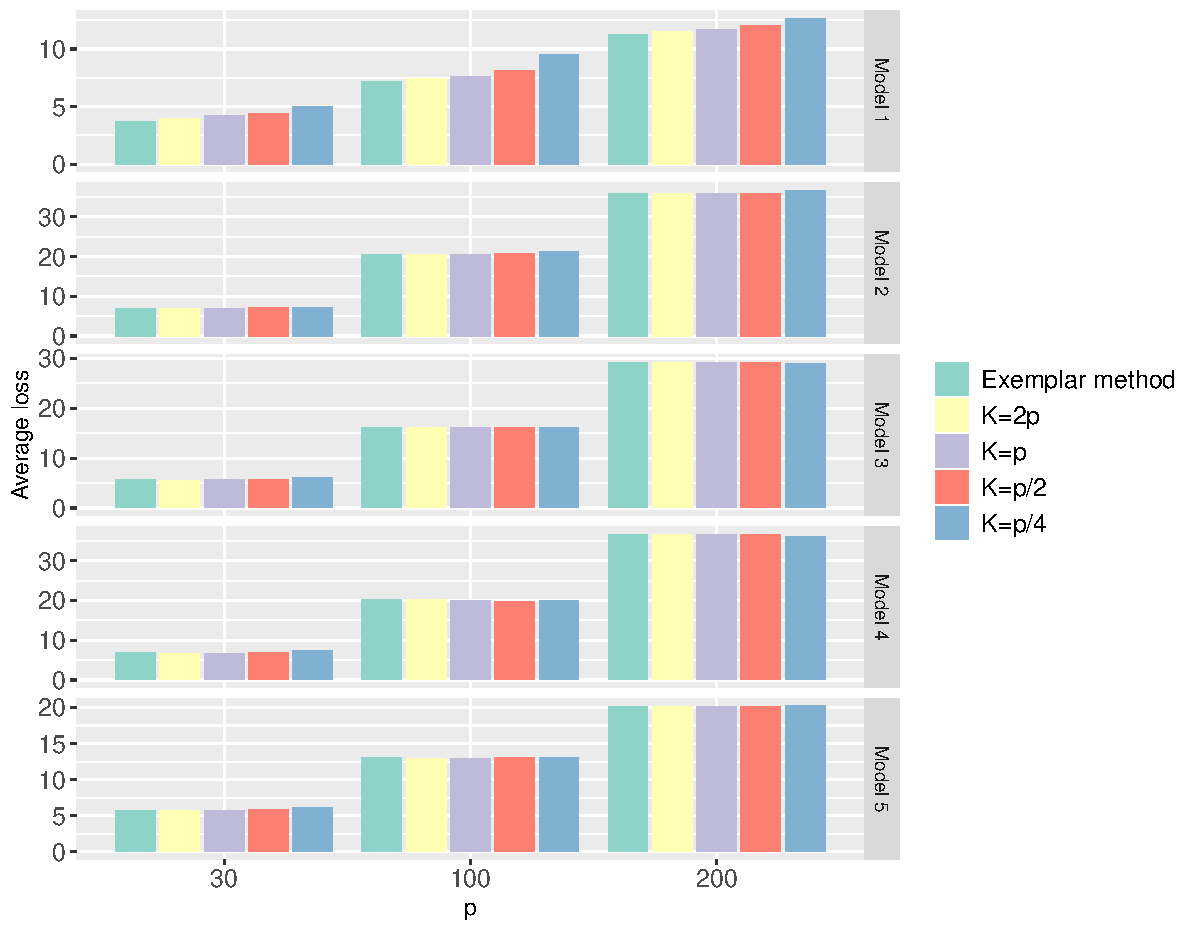
\includegraphics[width=0.85\textwidth]{img/sim1_frobenius.pdf} }
\end{center}
\caption{Average Frobenius norm errors over 200 replications. The Sparse, Block, Dense, Dense2, and Orth panels correspond to Models 1 through 5, respectively.}
\label{fig:sim1_frobenius}
\end{figure}

\begin{table}
\begin{center}
\caption{\label{tab:sim1_time} Average running time for different ratios.}
%\setlength{\tabcolsep}{3pt} % Default value: 6pt
\begin{tabular}{lrrr}
\Hline
            & p=30 & p=100 & p=200 \\
\hline
Exemplar method   & 0.0748          & 4.2575         & 47.8616       \\
$K=2p$	      & 0.0445 	     & 1.3166	   & 12.2612         \\
$K=p$            & 0.0291         & 0.8744         & 8.0862         \\
$K=p/2$         & 0.0207         & 0.5861         & 5.3757         \\
$K=p/4$      & 0.0153         &0.4132          & 3.7415         \\
\hline
\end{tabular}
\end{center}
\end{table}

Figure \ref{fig:sim1_frobenius} presents the Frobenius norm error estimates from Model 1 to Model 5. Table \ref{tab:sim1_time} shows the running time only for Model 1, because the running time does not vary much across different models. The results show that different $K$ exhibit similar performance and are comparable to the full exemplar method. Letting $K = p$ seemed to provide a good balance between accuracy and speed, so we implement our proposed method with $K = p$ in the rest of this paper.

\subsection{\label{compared}Methods compared}

In this section we refer to our approach using the abbreviation MSG: Matrix Shrinkage via $G$-modeling; we use MSGCor to refer to the version corrected for postive-definiteness. $K$-means clustering is applied on sample grids with $K=p$. We compared MSG and MSGCor to several existing high-dimensional covariance matrix estimation methods:

\begin{itemize}
\item Sample: the sample covariance matrix.
  
\item Linear: the linear shrinkage estimator of \citet{ledoit2004well} given in \ref{linear model}.
  
\item QIS: the Quadratic-Inverse Shrinkage estimator of \citet{ledoit2019quadratic}, a recently developed nonlinear shrinkage method. QIS performs linear shrinkage on the sample eigenvalues of the covariance matrix in inverse eigenvalue space. A bandwidth parameter is required, which we choose following the paper's recommendation.
  
\item NERCOME: the Nonparametric Eigenvalue-Regularized COvariance Matrix Estimator of \citet{lam2016nonparametric}. This nonlinear shrinkage method randomly splits the samples into two groups, one for estimating eigenvectors and the other for estimating eigenvalues. Combining the estimates gives a matrix. Following the article, we repeated this procedure 50 times and took the final covariance matrix estimator to be the average of the individual matrices.
  
\item Adap: the adaptive thresholding method of \citep{cai2011adaptive} for sparse covariance matrices, which applies soft thresholding to entries of the sample covariance matrix. The threshold method is adaptive to the entry's variance and involves a tuning parameter. We fixed the parameter at 2, as recommended.
\end{itemize}

In addition to the above estimators, we also implemented the two following oracle estimators, which cannot be implemented in practice as they require the unknown $\bs{\Sigma}$.
\begin{itemize}
\item OracNonlin: the optimal rotation-invariant covariance estimator, defined in \citet{ledoit2019quadratic}, with $\bs{\Sigma} = \bs{U}^T\text{diag}(\bs{l})\bs{U}$, where $\bs{U}=(\bs{u}_1\ldots\bs{u}_p)$ is the sample eigenvector matrix and $\bs{l} = (d_1, \ldots, d_p)$ is composed of oracle eigenvalues $d_i = \bs{u}_i^T\bs{\Sigma} \bs{u}_i$. The sample covariance, the linear shrinkage estimator of \citet{ledoit2004well}, and the nonlinear shrinkage estimators QIS and NERCOME are all rotation-invariant.
  
\item OracMSG: the optimal covariance estimator in the class of separable estimators $\mathcal{S}$ \ref{separable}. It equals our proposed estimator \ref{proposed} except with the true $G_p$ \ref{bayesian} instead of $\widehat{G}_p$ \ref{Gp hat}. The adaptive thresholding method of \citet{cai2011adaptive} also targets a separable estimator.
\end{itemize}

\begin{figure}
\begin{center}
\centerline{  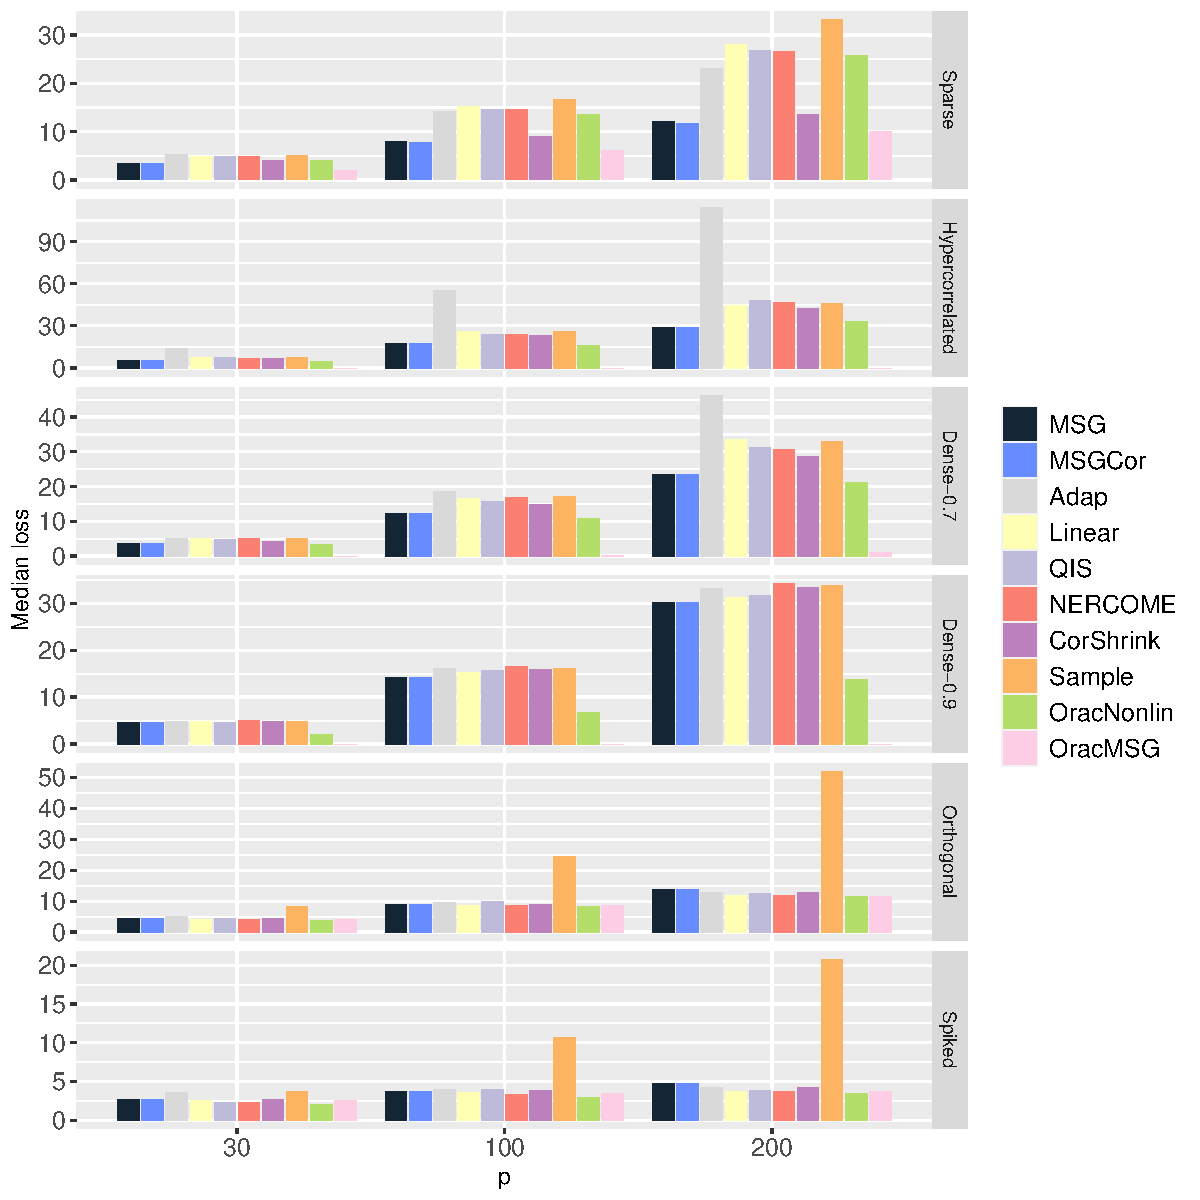
\includegraphics[width=0.85\textwidth]{img/sim2_frobenius.pdf}}
\end{center}
\caption{Average Frobenius norm errors over 200 replications. The Sparse, Block, Dense, Dense2, and Orth panels correspond to Models 1 through 5, respectively. In MSG, $K$-means clustering is applied with $K=p$}
\label{fig:sim2_frobenius}
\end{figure}


Figure \ref{fig:sim2_frobenius} presents the Frobenius loss for different estimators. Our MSG methods had the lowest or near-lowest errors across all settings except for Model 4 which has high correlations 0.9. This is not surprising because our method assumed independence of $\bs{A}_{jk}$.  In some cases, for example in Models 1 and 2, the improvement was substantial. Model 2 was especially interesting because the standard deviation and correlations were related. Our proposed empirical Bayes estimator was able to capture this dependence in its estimate of the prior $G_p$ \ref{bayesian} and leverage it to provide much more accurate estimates. The nonlinear shrinkage estimators very slightly outperformed MSG in Model 5. In every setting, correcting MSG for positive-definiteness never increased the risk and decreased the risk in some cases. We also did experiments for Spectral norm and Matrix $\ell_1$. The results for this two norms are very similar to Frobenius norm. One exception is Adap has the lowest error in terms of Matrix $\ell_1$ norm in Model 1 because of its sparsity. Though our estimator was motivated in terms of the Frobenius norm error, it performed extremely well in terms of the other two norms as well.

Finally, the simulations show that the class of separable estimators \ref{separable} proposed in this paper is fundamentally different from the class of rotation-invariant estimators, as the oracle optimal estimators in these two classes behave very differently. For example, the oracle separable estimator had vanishing risk in Model 2, while the oracle rotiation-invariant estimator does not. Separable estimators seemed better for Models 1 and 2 while rotation-invariant estimators were superior in Models 3 and 4. They seem comparable in Model 5.

\subsection{Data analysis}
\label{gene analysis}
Covariance matrix estimation is often used to reconstruct gene networks \citep{markowetz2007inferring}. We applied our MSG and the other covariance matrix estimators described in Section \ref{compared} to gene network estimation using data from a small round blue-cell tumor microarray experiment \citep{khan2001classification}, which was also studied by \citet{cai2011adaptive}. \citet{osareh2009classification} report the expression of 2308 genes from 63 samples from four groups: 12 neuroblastoma, 20 rhabdomyosarcoma, 8 Burkitt lymphoma, and 23 Ewing's sarcoma patients. In MSG, the clustering parameter $K$ is still set as $p=200$. We followed the same data preprocessing as \citet{cai2011adaptive} and sorted the genes in decreasing order according to their $F$-statistic
\begin{equation}
F = \frac{1}{k-1}\sum_{m=1}^kn_m(\overline{x}_m - \overline{x})^2 /   \frac{1}{n-k}\sum_{m=1}^k (n_m-1)\widehat{\sigma}_m^2 
\end{equation}
where $k = 4$ is the number of patient categories, $n_m$, $\overline{x}_m$, and $\widehat{\sigma}_k$ represent the sample size, sample mean, and sample variance of the gene's expression in the $m$th category, respectively, and $\overline{x}$ is the global mean. We proceeded with the top 40 genes and bottom 160 genes.

We applied various methods to estimate the covariance matrix of these 200 genes. To measure the accuracy of the estimators, we split the 63 samples into two subsets $\bs{X}_1$ and $\bs{X}_2$, ensuring that each subset consisted of the same number of subjects from each of the four disease groups. After centering the variables to have zero mean, we used $\bs{X}_1$ to calculate covariance matrix estimates and compared these to the sample covariance matrix $\bs{S}_2$ of $\bs{X}_2$, which served as a proxy for the unknown true covariance matrix. We measured the errors using the Frobenius, spectral, and matrix $\ell_1$ norms. We repeated this process 200 times.

Table \ref{tab:tab1} reports the average errors across the replications. Our MSG methods had the lowest average error. The positive-definiteness correction slightly reduced the risk as well. The linear shrinkage estimate was almost as accurate, but the other methods were much less accurate. These results suggest that our estimator can perform well in realistic settings, where the mean-zero multivariate normal distributional assumption on the data may not be met.

\begin{table}
\begin{center}
\caption{\label{tab:tab1} Average gene expression covariance matrix estimation errors. Bold entries highlight the smallest errors in each column.}
%\setlength{\tabcolsep}{3pt} % Default value: 6pt
\begin{tabular}{lrrr}
\Hline
            & Frobenius & Spectral & Matrix $\ell_1$ \\
\hline
MSG   & 24.07          & 12.89         & 47.12         \\
MSGCor & \textbf{23.90} & \textbf{12.87}& \textbf{46.63}         \\
Adap        & 28.81          & 17.20         & 50.71         \\
Linear      & 24.59         & 13.57         & 51.43         \\
QIS         & 28.66          & 15.94         & 59.30         \\
NERCOME     & 29.76          & 20.13         & 57.30         \\
Sample      & 28.39          & 16.10         & 57.90         \\
\hline

\end{tabular}
\end{center}
\end{table}

In addition to comparing the numerical accuracies, we also investigated whether our estimator gave qualitatively different gene networks compared to the other approaches. First, Figure \ref{network} illustrates the covariance matrices in network form, where each node represents a gene and each edge represents a non-zero covariance between the genes it connects. To avoid completely connected graphs, we sparsified the matrix estimates by thresholding the smaller entries of each matrix to zero. Since the adaptive thresholding method of \citet{cai2011adaptive} naturally produced a sparse estimated matrix, we thresholded the other matrix estimates to match the sparsity level of the \citet{cai2011adaptive} estimate.

\begin{figure}
\begin{center}
\centerline{ 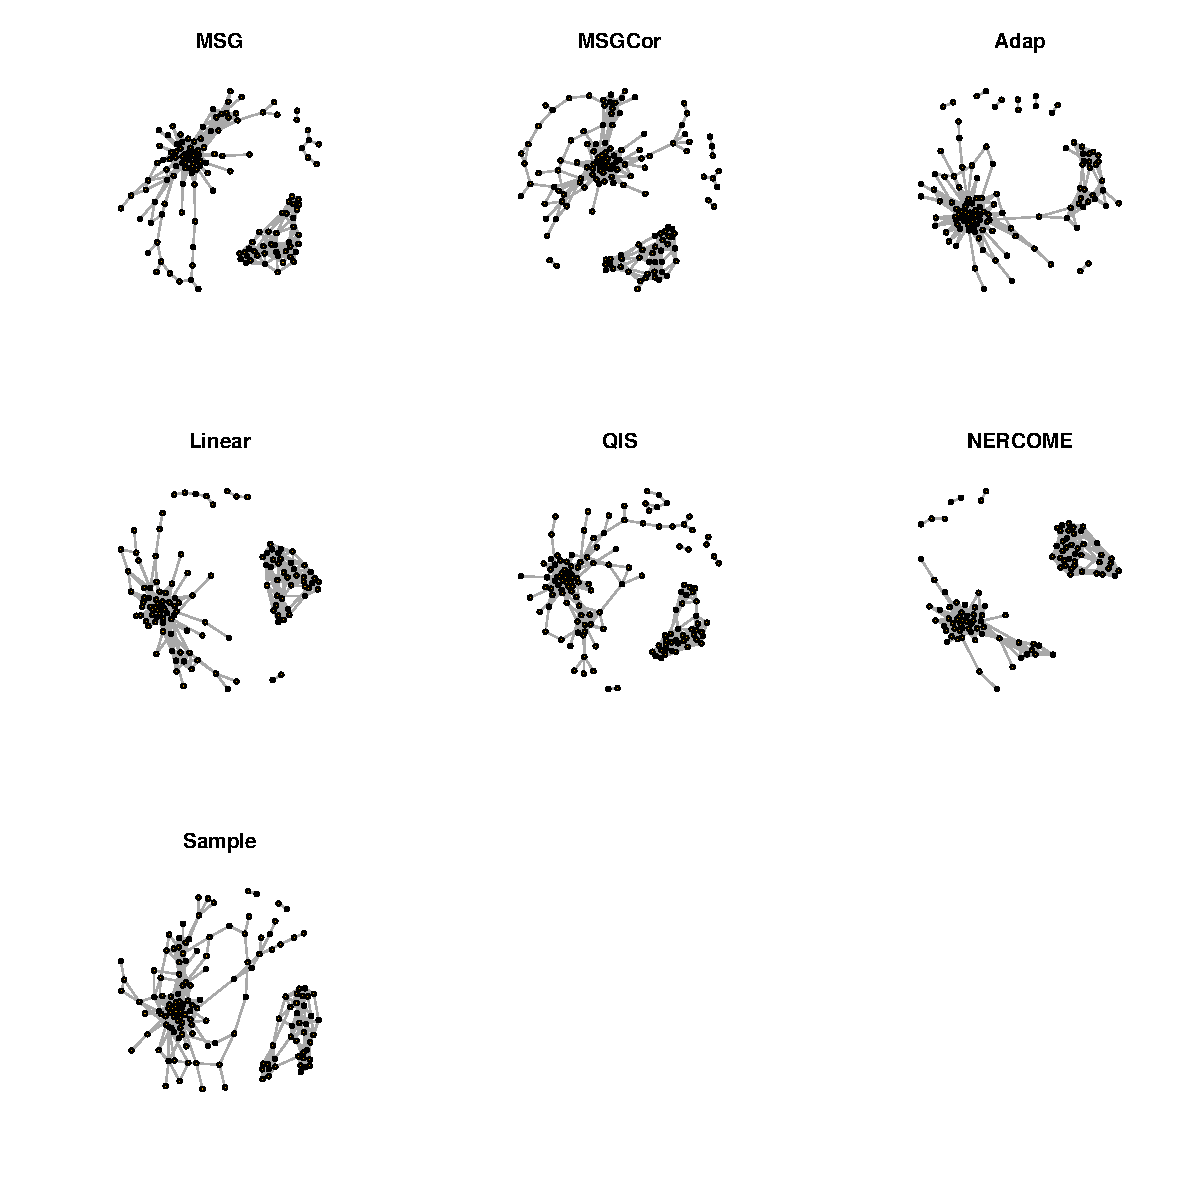
\includegraphics[width=0.85\textwidth]{img/network.pdf}}
\end{center}
\caption{Gene networks recovered by the different covariance matrix estimation methods.}
\label{network}
\end{figure}

The results show several interesting features. First, there appear to be two major clusters, which are disconnected in every estimated network except for the one produced by the adaptive thresholding approach. Second, the larger cluster appears to contain two sub-clusters, and this finer structure was only recovered by MSG and QIS, and to a lesser extent the linear shrinkage estimator and NERCOME. Finally, the nodes in the networks estimated by QIS and NERCOME appear to be clustered more tightly together compared to in the other networks. These observations suggest that MSG produces qualitatively different networks, in addition to lower estimation errors.

Finally, we also compared the estimated degrees of the genes in the different networks. For each estimated network, we ordered the 200 genes by degree and then selected the top 20\%, denoting this set $J_k$ for the $k$th network. For each pair of networks $k$ and $k'$, we calculated the similarity between their most connected genes using Jaccard index $\vert J_k \cap J_{k'} \vert / \vert J_k \cup J_{k'} \vert$. Figure \ref{top20} visualizes these similarities. Interestingly, however, among all estimators, they were also the most similar to the unbiased sample covariance matrix. Together with the above results, this indicates that MSG may simultaneously give the lowest error and, at least in terms of degree estimation, the most unbiased results.

\begin{figure}
\begin{center}
\centerline{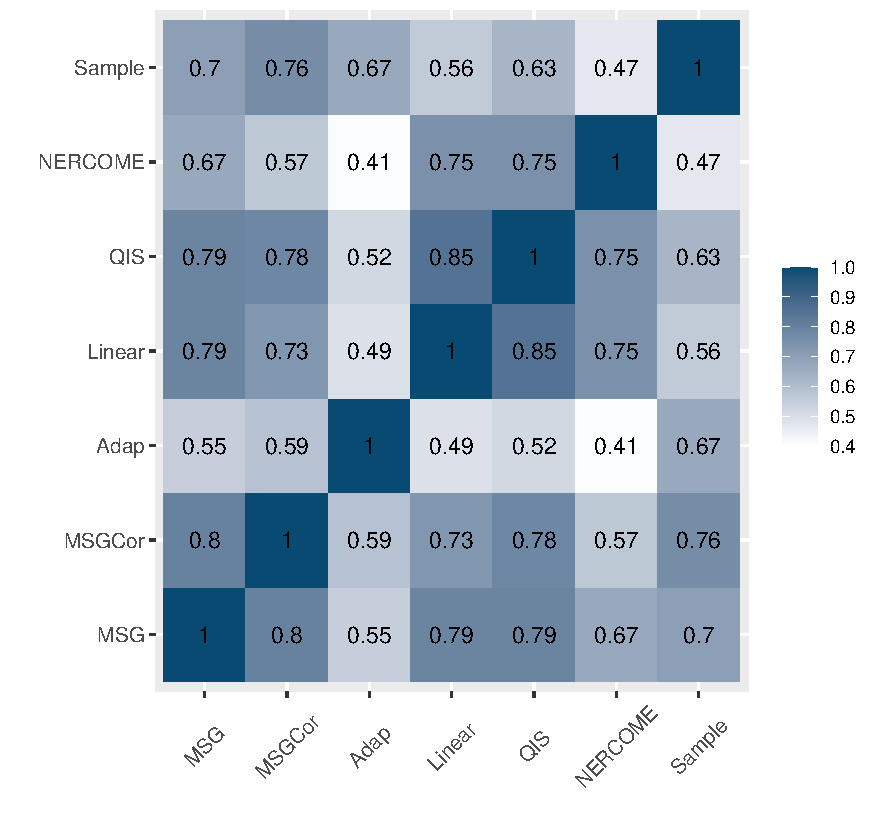
\includegraphics[width=0.85\textwidth]{img/top20.pdf}}
\end{center}
\caption{Similarities of gene degrees between the estimated networks. Each number reports the Jaccard index between the top 20\% most connected genes of each pair of networks.}
\label{top20}
\end{figure}

\section{\label{sec:discussion}Discussion}
\label{discussion}

The class of separable covariance matrix estimators \ref{separable} that we proposed in this paper appears to be very promising. Many existing procedures already explicitly or implicitly target this class, and our proposed estimate \ref{proposed} of the optimal separable estimator outperforms a number of existing covariance matrix estimators. This is surprising because our approach vectorizes the matrix and therefore cannot take matrix structure, such as positive-definiteness, into account. This suggests that a vectorized approach combined with a positive-definiteness constraint may have improved performance. The resulting estimator would necessarily not be separable, because the estimate of the $jk$th entry would depend on more than just the $j$th and $k$th observed features, so the $g$-modeling estimation strategy is insufficient. More work is needed.

Though our estimator performs well in simulations and in real data, providing theoretical guarantees is difficult. In the standard mean vector estimation problem with $Y_i \sim N(\theta_i, 1)$, \citet{jiang2009general} showed that an empirical Bayes estimator based on a nonparametric maximum likelihood estimate of the prior on the $\theta_i$ can indeed asymptotically achieve the same risk as the oracle optimal separable estimator. However, this was in a simple model with a univariate prior distribution. \citet{saha2020nonparametric} extended these results to multivariate $\bs{Y}_i \sim N(\bs{\theta}_i, \bs{\Sigma}_i)$ with a multivariate prior on the $\bs{\theta}_i$, but assumed that the $\bs{Y}_i$ were independent. In contrast, our covariance matrix estimator is built from arbitrarily dependent $\bs{A}_{jk}$. These imposes significant theoretical difficulties that will require substantial work to address; we leave this for future research.

Finally, we have so far assumed that our data multivariate normal. To extend our procedure to non-normal data belonging to a parametric family, we can simply modify the density function $f(\cdot \mid \bs{\eta})$ in the nonparametric maximum compositive likelihood problem \ref{Gp hat} and in our proposed estimator \ref{proposed}. If $f$ is unknown or difficult to specify, alternative procedures may be necessary to approximate the optimal separable rule.

\backmatter

\section*{Acknowledgments}
We thank Dr. Roger Koenker for his valuable comments.\vspace*{-8pt}


\bibliographystyle{biom} 
\bibliography{biblio}

\section*{Supporting Information}
Web Appendices, Tables, and Figures referenced in Section 3 are available with this paper at the Biometrics website on Wiley Online Library.

\appendix
\section{}
\subsection{Proof of Proposition \ref{prop:linear}}

\begin{proof}
  We first rewrite the risk estimate $\widehat{R}(\beta_S, \beta_I)$. Define $\bs{M}=(\sum_{j,k=1}^p\widehat{\Delta}_{jk}^2, 0)^\top$, $\bs{\beta} = (\beta_S, \beta_I)^\top$, and the vectorized covariance matrices $\bs{v_S}=(s_{11},\ldots, s_{pp})^\top $, $\bs{v_I}=(u_{11},\ldots, u_{pp})^\top $, and $\bs{v_{\Sigma}} = (\sigma_{11},\ldots,\sigma_{pp})^\top$. Then the unbiased risk estimator can be re-written as
  \[
  \widehat{R}(\beta_S,\beta_I) = \bs{\beta}^\top (\bs{Z}^\top \bs{Z})\bs{\beta} - 2(\bs{Z}\bs{v_S}-\bs{M})^\top \bs{\beta} - \bs{1}^\top \bs{M},
  \]
  where $\bs{Z} =(\bs{v_S}, \bs{v_I})$. Therefore
  \begin{align*}
    \widehat{\bs{\beta}} &= \arg\min_{ \bs{\beta} }(\bs{Z}^\top \bs{Z})^{-1}(\bs{Z}\bs{v_S}-\bs{M}),\\
    &
    \widehat{\bs{v}}_{\bs{\Sigma}} = \bs{Z\widehat{\beta}} = \bs{v_S} - \bs{Z}(\bs{Z}^\top \bs{Z})^{-1}\bs{M}.
  \end{align*}

  We will need to show $\widehat{\mu} b_n^2 / d_n^2 = \widehat{\beta}_I$ and $\widehat{\beta}_I/\widehat{\mu} + \widehat{\beta}_S = 1$. Since
$$\bs{Z}^\top \bs{Z} = \begin{pmatrix}
s_{11} &\ldots &s_{pp} \\
u_{11} &\ldots &u_{pp} 
\end{pmatrix}\begin{pmatrix}
s_{11}  &u_{11} \\
\ldots&\ldots\\
s_{pp} &u_{pp} 
\end{pmatrix}=\begin{pmatrix}
\sum_{j,k=1}^ps_{jk}^2 & \sum_{j=1}^ps_{jj}\\
\sum_{j=1}^ps_{jj} & p
\end{pmatrix}$$
and
$\text{det}( \bs{Z}^\top \bs{Z} ) = p\sum_{j,k=1}^ps_{jk}^2 - (\sum_{j=1}^p s_{jj})^2 = p^3d_n^2$, it follows that
$$(\bs{Z}^\top \bs{Z})^{-1} = \frac{1}{p^3d_n^2}\begin{pmatrix}
p & -\sum_{j=1}^p s_{jj}\\
-\sum_{j=1}^p s_{jj} & \sum_{j,k=1}^ps_{jk}^2
\end{pmatrix},$$
and in addition
$$\bs{Z}^\top \bs{S} = \begin{pmatrix}
\sum_{j,k=1}^ps_{jk}^2\\
\sum_{j=1}^p s_{jj}
\end{pmatrix},
\quad 
\bs{Z^\top S}-\bs{M} =  \begin{pmatrix}
&\sum_{j,k=1}^ps_{jk}^2 - \widehat{\Delta}_{jk}^2\\
&\sum_{j=1}^p s_{jj}
\end{pmatrix}.$$

Therefore
\begin{align*}
\widehat{\bs{\beta}}& = (\bs{Z}^\top \bs{Z})^{-1} \bs{Z^\top S} \\
&= \frac{1}{p^3d_n^2}\begin{pmatrix}
p & -\sum_{j=1}^p s_{jj}\\
-\sum_{j=1}^p s_{jj} & \sum_{j,k=1}^ps_{jk}^2
\end{pmatrix}\begin{pmatrix}
\sum_{j,k=1}^ps_{jk}^2 - \widehat{\Delta}_{jk}^2\\
\sum_{j=1}^p s_{jj}
\end{pmatrix}\\
&= \frac{1}{p^3d_n^2}\begin{pmatrix}
 p\sum_{j,k=1}^p s_{jk}^2 -p\sum_{j,k=1}^p\widehat{\Delta}_{jk}^2-(\sum_{j=1}^ps_{jj})^2\\
 (\sum_{j=1}^ps_{jj}) (\sum_{j,k=1}^p\widehat{\Delta}_{jk}^2)
\end{pmatrix}.
\end{align*}
The second component of $\widehat{\bs{\beta}}$ equals $\widehat{\beta}_I$, so
\begin{align*}
\widehat{\beta}_I &= \frac{1}{p^3d_n^2} (\sum_{j=1}^ps_{jj}) (\sum_{j,k=1}^p\widehat{\Delta}_{jk}^2)\\
&=\{(\sum_{j=1}^ps_{jj})/p\}   \{(\sum_{j,k=1}^p\widehat{\Delta}_{jk}^2)/p^2 \} / d_n^2
=\widehat{\mu}\frac{b_n^2}{d_n^2}.
\end{align*}
Furthermore,
\begin{align*}
\widehat{\beta}_I /\widehat{\mu} + \widehat{\beta}_S &= \frac{1}{p^3d_n^2}p\sum_{j,k=1}^p \{s_{jk}^2 -p\sum_{j,k=1}^p\widehat{\Delta}_{jk}^2-(\sum_{j=1}^ps_{jj})^2+p\sum_{j,k=1}^p\widehat{\Delta}_{jk}^2\}\\
&=\frac{1}{p^3d_n^2}\{p\sum_{j,k=1}^p s_{jk}^2 -(\sum_{j=1}^ps_{jj})^2\}
=
1.
\end{align*}
\end{proof}

\label{lastpage}
\end{document}
